Através das reuniões da equipe de requisitos com o cliente, foram identificados aspectos inerentes ao funcionamento
atual do Corpo de Bombeiros Militar do Distrito Federal (CBMDF). Esses aspectos foram agrupados e deram origem a causas, estas
que ajudaram a identificar o problema do CBMDF.

As causas citadas foram representadas, junto ao problema, em um diagrama de causa e evento na figura \ref{fishbone}.

  \begin{figure}[!htbp]
    \centering
    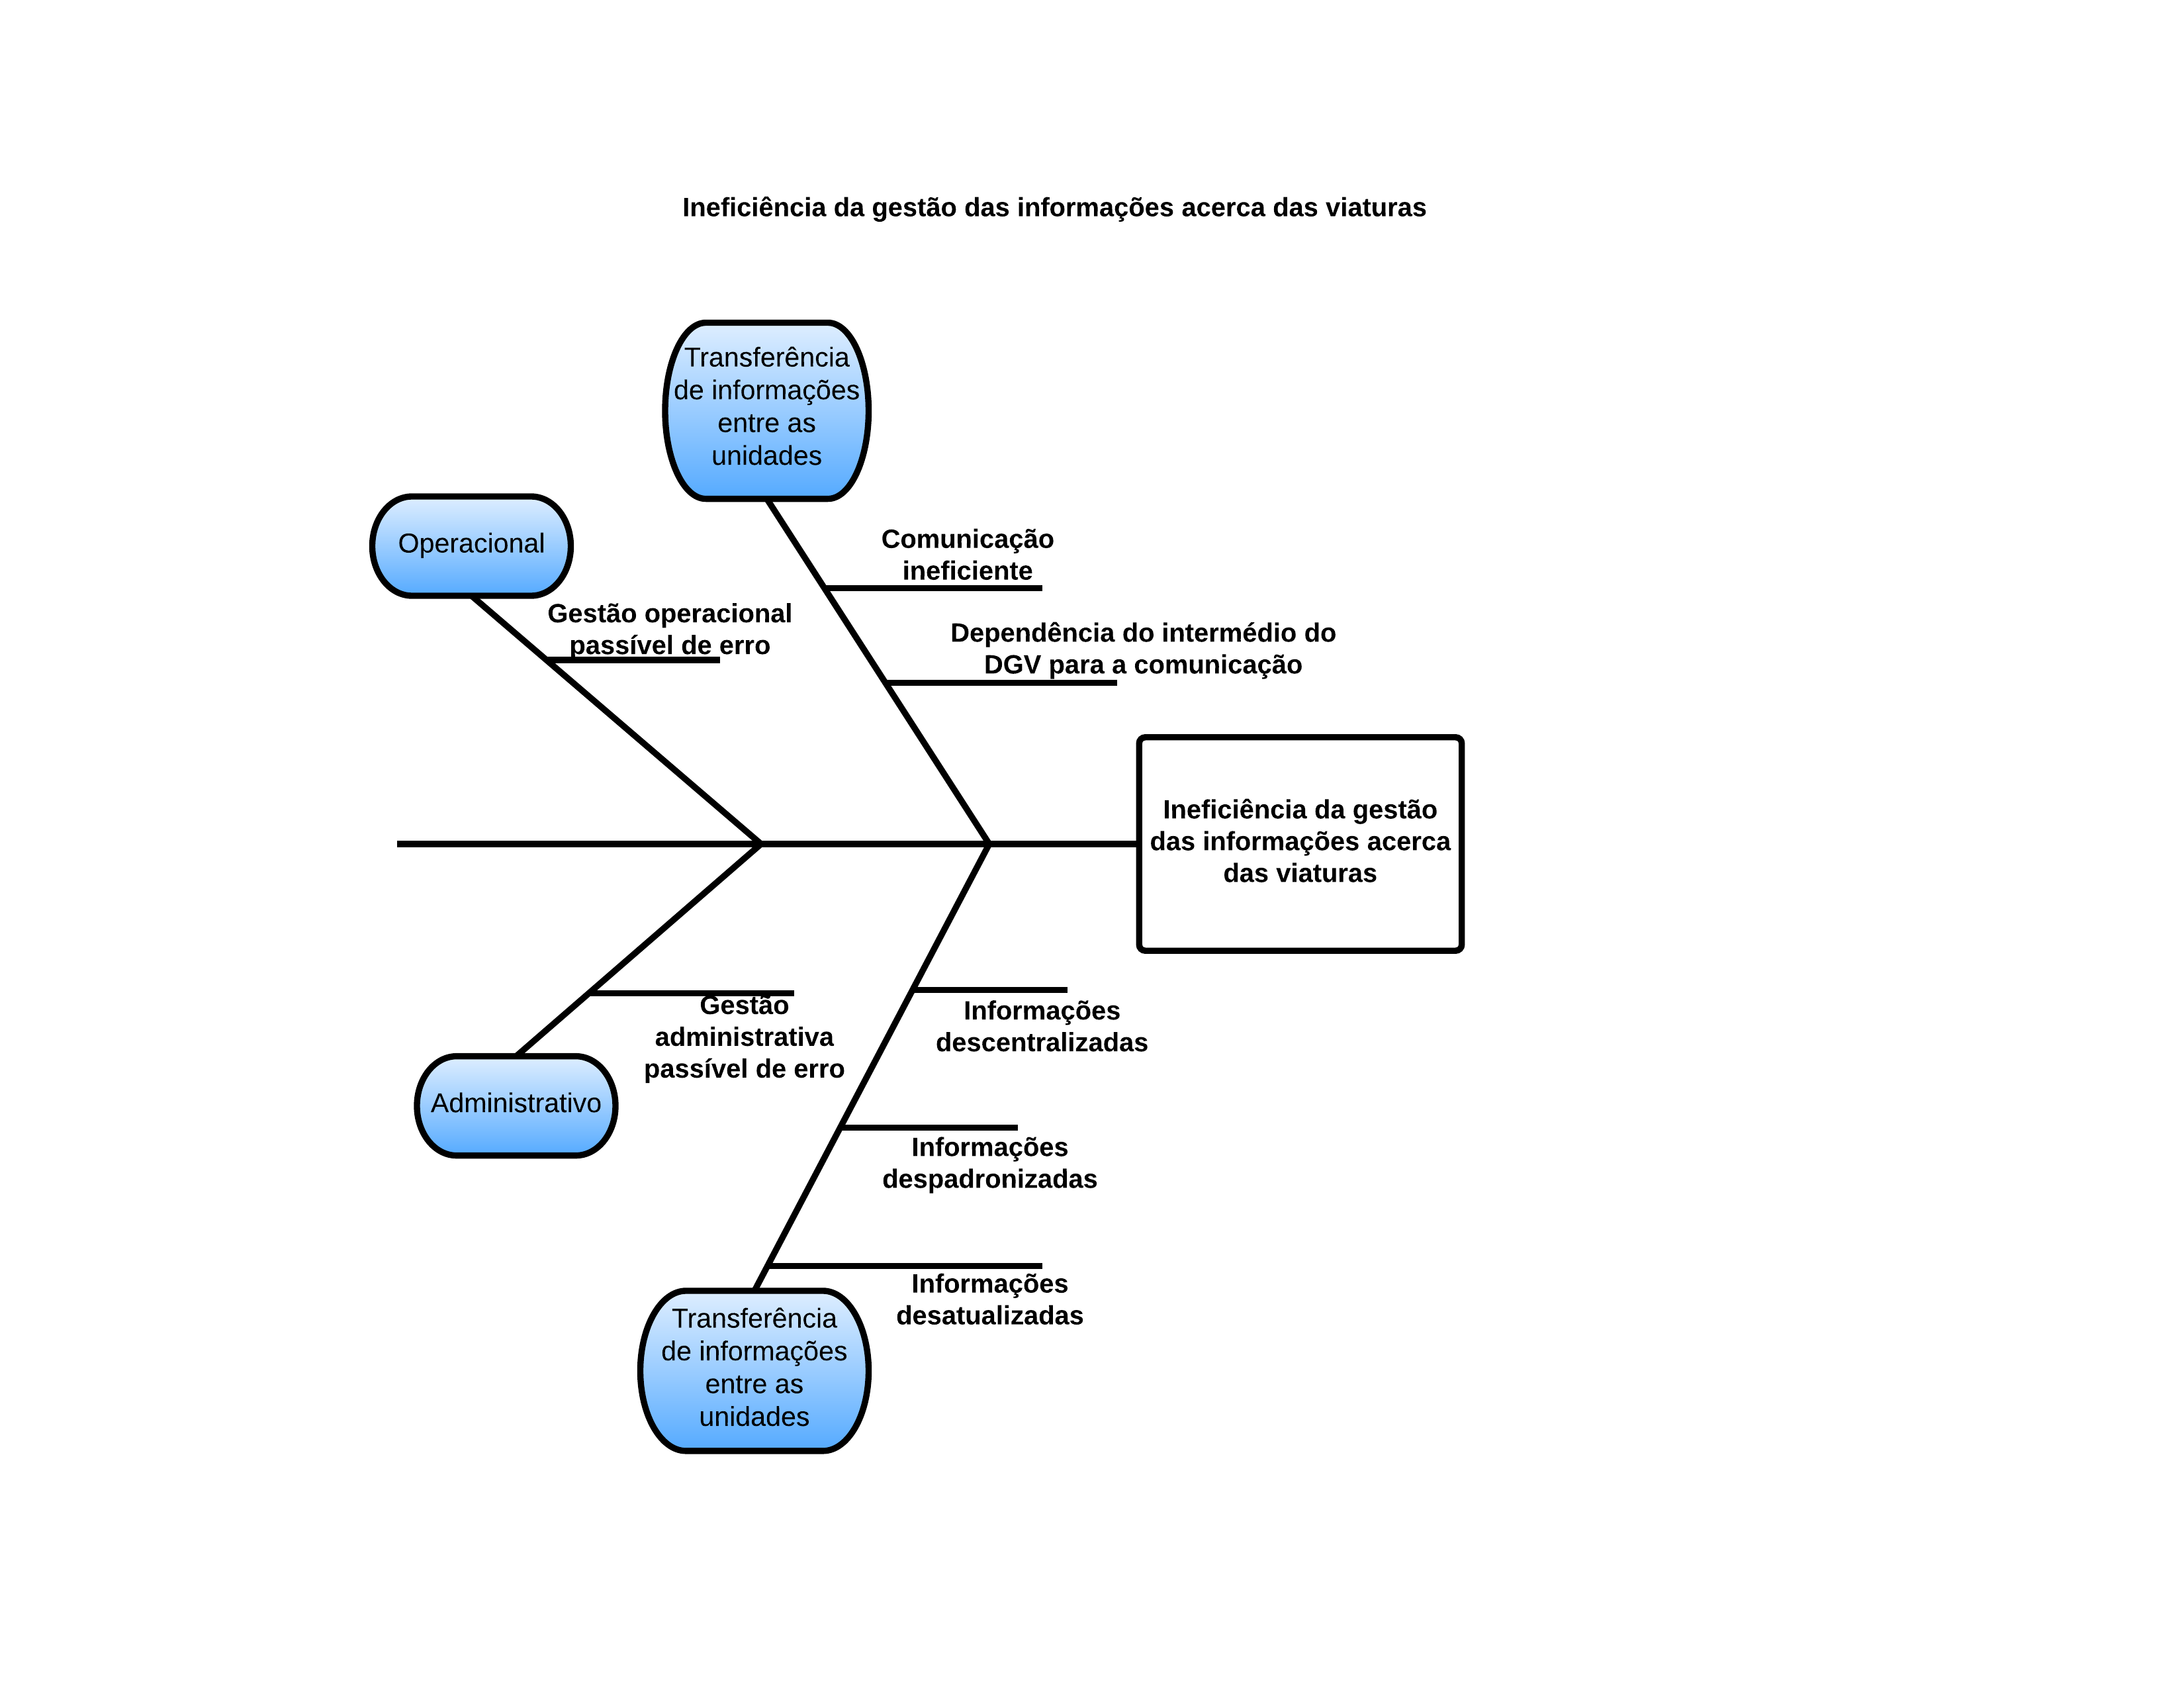
\includegraphics[scale=0.8, angle=0]{figuras/fishbone}
    \caption{Diagrama de causa e evento (\textit{fishbone}) com as causas e problema do CBMDF.}
    \label{fishbone}
  \end{figure}

    \vfill
  \pagebreak

Para uma descrição mais clara e formal do problema, foi utilizado o seguinte \textit{framework} de descrição de problema:

  \textbf{O problema:} Ineficiência da gestão das informações acerca das viaturas.
  
  \textbf{Afeta:} Corpo de Bombeiros Militar do Distrito Federal.
  
  \textbf{Cujo impacto é:} Tomadas de decisões inadequadas, falta de qualidade de vida para os bombeiros e 
  gastos desnecessários.
  
  \textbf{Uma solução bem sucedida seria:} Um sistema que centralizaria as informações acerca das viaturas, as fornecendo 
  em tempo real para quem necessitasse das mesmas.
  
  \vfill
  \pagebreak